\documentclass{sig-alternate}
\usepackage{verbatim}
\usepackage{array}
\usepackage{caption}
\usepackage{subcaption}

\newtheorem{definition}{Definition}
\begin{document}
%
% --- Author Metadata here ---
\conferenceinfo{SIGIR}{'2016 Pisa, Italy}

\title{Detecting significant events in news corpora}

\maketitle
\begin{abstract}
Retrospective event identification is the task of identifying and summarizing significant events in time-stamped corpora. In this short paper, we present a simple unsupervised method for identifying significant events in a news corpus based on feature temporal mutual information ($I_t$) and non-negative matrix factorization (NMF). We evaluate our method using a preliminary test collection and evaluation methodology that can be used for future comparative research. We compare our method to a latent Dirichlet allocation (LDA) approach to better understand the differences between events and topics.

\end{abstract}

% A category with the (minimum) three required fields
\category{H.3.3}{Information Search and Retrieval}{}

\terms{}

\keywords{Event detection}

\section{Introduction}

Imagine a Wikipedia editor creating the `year' page (e.g., 1988) containing a list of important events that occurred during that year. Given a corpus of news articles (or other timestamped collection), it should be possible to show the editor a list of major events that were reported during the time period to facilitate the creation or validation of these pages. Such a system might rank the events by importance, provide estimated dates of event occurrence, and a ranking of candidate Wikipedia pages that describe the associated event. 

In this short paper, we present a novel method for retrospective event identification in news corpora based on temporal mutual information \cite{Teng2008} and non-negative matrix factorization \cite{Lee2001}. We also introduce a preliminary test collection and evaluation methodology based on Wikipedia that can be used for future comparative research.  As far as we know, we are the first to propose a method for comparative evaluation in this type of retrospective event identification task.

The results of our method are compared to a baseline implementation\footnote{Although we contacted the authors, we were unable to gain access to the original source code. We acknowledge that our implementation may not be exactly as described in the original article due to some ambiguities in the original model description.} of the model described in \cite{He2007}. Our model outperforms the baseline ...


\section{What is an event?}

The concepts of `event detection' or `event extraction' are common in the information retrieval and natural language processing literature. In this paper, we are concerned with the retrospective identification of large-scale events as reported in historical news corpora. A number of studies have used the concepts of ``significant,'' ``seminal,'' or ``newsworthy'' events to describe such large-scale events.  Our notion of event is most closely related to the ``seminal events'' of the Topic Detection and Tracking (TDT) task, although the task itself is quite different. Examples of large-scale events include major elections, natural disasters, political revolutions, wars, and acts of violence.


\section{Related Work}

Recent studies in retrospective event identification apply feature-centric models \cite{Yi, Fung2005, Chen2009, Teng2008, Weng2011} that first identify interesting terms (or features) which are subsequently grouped or combined to represent events. 

For example, Fung et al \cite{Fung2005} identify temporally interesting features using a series of binomial distributions. The terms are subsequently combined  into events using a cost-minimization approach that balances the similarity of the temporal distributions of terms and the co-occurrence of terms in documents. 

Weng and Lee \cite{Weng2011} use wavelet analysis to identify interesting features and then apply graph partitioning to a graph with terms as nodes and the cross-correlation of term time-series as edge weights. This approach does not account for term co-occurrence in documents.

He, Chang and Lim \cite{He2007} use spectral analysis to identify interesting features in text corpora. Features are grouped into events using a cost-minimization approach that combines the similarity of the temporal distributions using KL divergence and co-occurrence of terms in documents. We use this model as a baseline for comparison.

Also related to the current study is research in latent semantic analysis (LSA) \cite{Deerwester1990, Hofmann1999} and topic modeling \cite{Blei2003}.  Event models can be seen as a special type of temporally-constrained topic models. Our approach is akin to the factor-based LSA model, but we anticipate expanding this work to a generative probabilistic framework in the future.  




\section{Event detection model}

Each of the feature-centric models described above includes two basic steps. The first is to identify terms or features that are indicative of an event in the corpus, generally using time-series methods. The second is to combine terms generated by the same underlying event into event models.  This is usually done by balancing temporal similarity (e.g., time series correlation) with term co-occurrence in documents.

In this study, we identify temporally interesting terms using the first-order autocorrelation (ACF) of the term time series \cite{Jones2007}. We then calculate the temporal mutual information between the top $K$ terms based on ACF and apply non-negative matrix factorization (NMF) to identify latent factors. We interpret the resulting factors as events. The basic process is defined as follows:

First, we construct a temporal index from the document collection that consists of time series for each term in the vocabulary at a particular interval (e.g., hour, day, week):
\begin{definition}
 \text{ \normalfont Feature time series. }
 The time series of a feature f is defined as the sequence:
\[
y_f = [y_f(1), y_f(2), ..., y_f(T)],
\]
where each element $y_f(t)$ is a measure of feature f at time t. For this paper, we use the simple document frequency:
\[
	y_f(t) = DF_f(t)
\]
where $DF_f(t)$ is the number of documents containing feature f at time t.
\end{definition}

Next, for each term in the vocabulary, we calculate the first-order autocorrelation ($\rho$) of the time series. 
\begin{definition}
 \text{ \normalfont First order autocorrelation. }
 Given 
\[
\rho = \dfrac{\sum_{i=1}^{N-1} (y_t - \bar{y}_{(1)})(y_{t+1} - \bar{y}_{(2)})}{ \big [ \sum_{i=1}^{N-1}  (y_t - \bar{y}_{(1)})^2 \big ] ^{1/2} \big [\sum_{i=1}^{N-1} (y_{t+1} - \bar{y}_{(2)})^2 \big ]^{1/2}}
\]
\end{definition}

Terms with high temporal dependency will have very high (1) or very low (-1) $\rho$.  For this short paper, we consider only the top $K$ features based on ACF, where $K$ is chosen heuristically.

For all terms with high temporal dependency, we calculate the temporal mutual information $I_t(x;y \vert t)$ between terms \cite{Teng2008}. 

\begin{definition}
 \text{ \normalfont Temporal mutual information. }
Given a timestamp $t$ and pair of terms $x$ and $y$, the temporal mutual information between $x$ and $y$ in $t$ is defined by:
\[
I_t(x;y \vert t) = p(x,y \vert t) \log \dfrac{p(x,y \vert t)}{p(x \vert t) p(y \vert t)}
\]
\end{definition}

In this study, $I_t(x;y \vert t)$ is calculated independently for each interval (as opposed to cumulatively, as described in \cite{Teng2008}).

Finally, we construct a symmetric matrix of the maximum $I_t$ between terms and apply NMF \cite{Lee2001} to identify latent factors. 
\begin{definition}
 \text{ \normalfont Non-negative matrix factorization.}
 Given a non-negative matrix $V$, NMF finds matrix factors $W$ and $H$ such that:
\[
V \approx WH
\]
\end{definition}

We interpret the matrix $W$ as latent event models, using the assigned weights as term weights. The top $N$ models are evaluated as described in a latter section. 

\section{Baseline LDA model}

As noted above, there is a relationship between event detection and topic modeling approaches, such as latent Dirichlet allocation \cite{Blei2003}. Although the basic LDA model does not explicitly incorporate time, some topics are generated by events -- particularly in news corpora.

We compare our event detection model to a baseline of LDA-generated topics, ranked by the first order autocorrelation (ACF) of a topic time-series. The time series of a topic $m$ is defined as the sequence:
\[
y_m = [y_m(1), y_m(2), ..., y_m(T)],
\]
where each element $y_m(t)$ is a measure of the topic $m$ at time $t$. For this paper, we use the sum of the document-topic probability from LDA:
\[
	y_m(t) = \sum_{d \in D} p(m \vert d, t)
\]

We calculate the topic time series ACF as above. The top $N$ topic models are evaluated as described in the next section. 

\begin{table*}[!htbp]
\small
\begin{tabular}{| l | p{1cm} | p{8cm} | p{6cm} | } \hline
{\bf ID} & {\bf Date} &  {\bf Description}  & {\bf Wikipedia URL} \\ \hline
19 & Mar 11 & Terrorists execute simultaneous attacks, with bombs in 4 rush-hour trains in Madrid, killing 191 people.	&  2004\_Madrid\_train\_bombings \\ \hline
42 & June 28 & The U.S. led coalition occupying Iraq transfers sovereignty to an Iraqi Interim Government.	& Iraqi\_sovereignty \\ \hline
57 & Sept 1 & Chechen terrorists take 1,128 people hostage, mostly children, in a school in the Beslan school hostage crisis. & Beslan\_school\_siege \\ \hline
76 & Nov 2 & United States presidential election, 2004: Republican incumbent President George W. Bush is declared the winner over his Democratic challenger, U.S. Senator John F. Kerry, in a close election. & United\_States\_presidential\_election,\_2004 \\ \hline
91 & Dec 26 & One of the worst natural disasters in recorded history hits Southeast Asia, when the strongest earthquake in 40 years, measuring 9.3 on the Richter scale, hits the entire Indian Ocean region, which generates an enormous tsunami that crashes into the coastal areas of a number of nations. & 2004\_Indian\_Ocean\_earthquake\_and\_tsunami \\ \hline
\end{tabular}
\caption{Example entries from the known-events list (Wikipedia 2004)}
\label{table.knownevents}
\end{table*}

\section{Evaluation}

The primary concern in the evaluation of feature-centric event detection models is how effective the model is at identifying events in the corpus. For this short paper, we propose an evaluation methodology based on Wikipedia and the pooled results of the systems under comparison.

Before evaluation, each system generates a set of $N$ candidate event models based on the test corpus. Each model contains a list of $k$ terms and associated weights. 

To develop a ground-truth of \emph{known-events}, we start with events listed in the Wikipedia `year' pages for the period of the test collection. The known-event list contains an event ID, description, date, and associated Wikipedia URL. The pooled candidate events from the systems are manually reviewed to identify any events missing from the known-events list.  Each candidate event is manually compared to the list and, if it is determined by the assessor to represent an event that does not exist in the list, it is added. At the end of this process, we have a list of unique known-events based on a combination of the Wikipedia year pages and the pooled results from the systems.  

To determine whether a system's candidate event represents a real event, we again turn to Wikipedia. We use the candidate event models as queries against Wikipedia, returning the top $k$ pages. We hypothesize that a high-quality event model will serve as an effective query to the external system. For each of the top $N$ candidate events, we count the number of known-event URLs returned at each depth (i.e., 1-10). We then compare the systems based on the proportion of known events identified in the top $N$ candidate events at each depth.


\subsection{Test collection}
News articles from the year 2004 in the New York Times Annotated Corpus \cite{Sandhaus2008} are used for evaluation. Only articles found in section A (available via document metadata) are considered and summary articles are ignored. Stopwords are removed using the standard Indri list. The resulting collection consists of 25,689 documents.

The ``known-events'' list is constructed using the process described in the previous section based on the ``Events'' section of the 2004 Wikipedia year page\footnote{https://en.wikipedia.org/wiki/2004\#Events} and the top $N=50$ candidate events from the two systems.  The final ``known-events'' list contains 140 unique events with associated Wikipedia URLs. Of these events, 95 are from the Wikipedia year page and the remaining 55 were added based on the pooled system results.  Selected entries from the known-events list are presented in Table \ref{table.knownevents}.

The systems are compared based on the proportion of the top $N=50$ candidate events that are found in the known-events list at each depth (1-10).

\section{Results}
The TMINMF model was run using the top 1000 features based on ACF and $k=50$ factors for NMF. The LDA model was run using the Mallet implementation with $k=100$ topics, an interval of 10 for hyperparameter optimization, and all other default values. Only the top $N=50$ LDA topics were considered as events for evaluation, based on topic time series ACF.


\begin{figure*}[!ht]
\centering
\begin{subfigure}{.5\textwidth}
  \centering
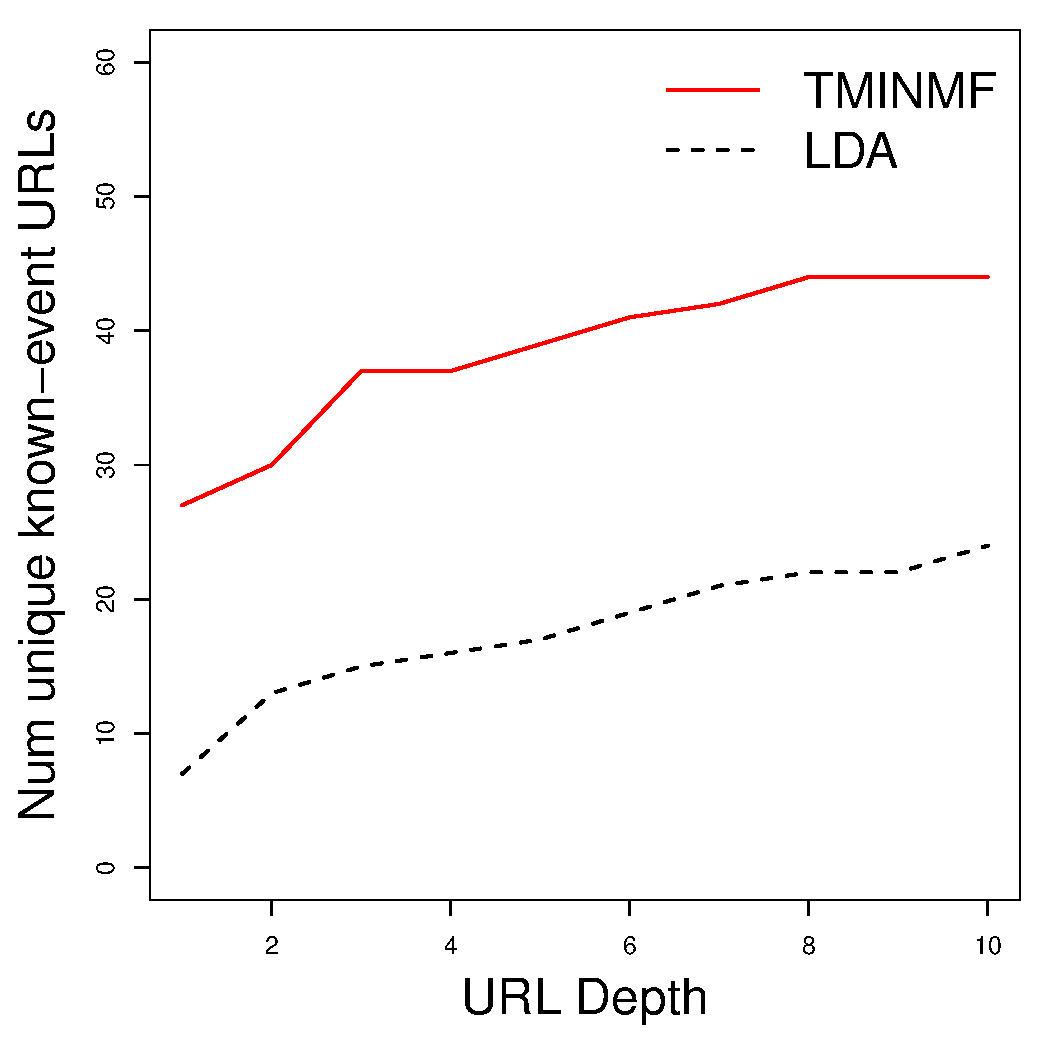
\includegraphics[width=10cm]{plots/events_at_depth.pdf}
\end{subfigure}%
\begin{subfigure}{.5\textwidth}
  \centering
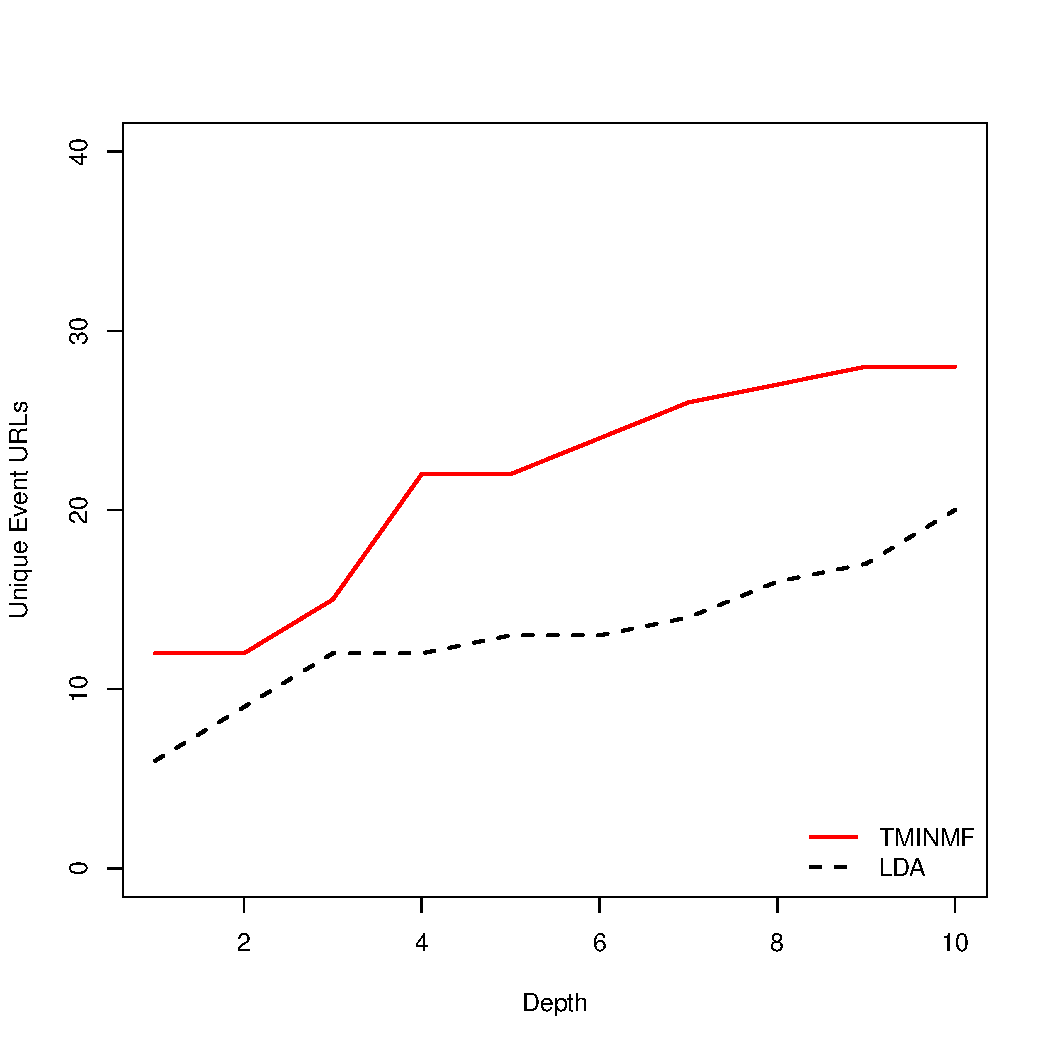
\includegraphics[width=10cm]{plots/unique_urls_at_depth.pdf}
\end{subfigure}
\begin{subfigure}{.5\textwidth}
  \centering
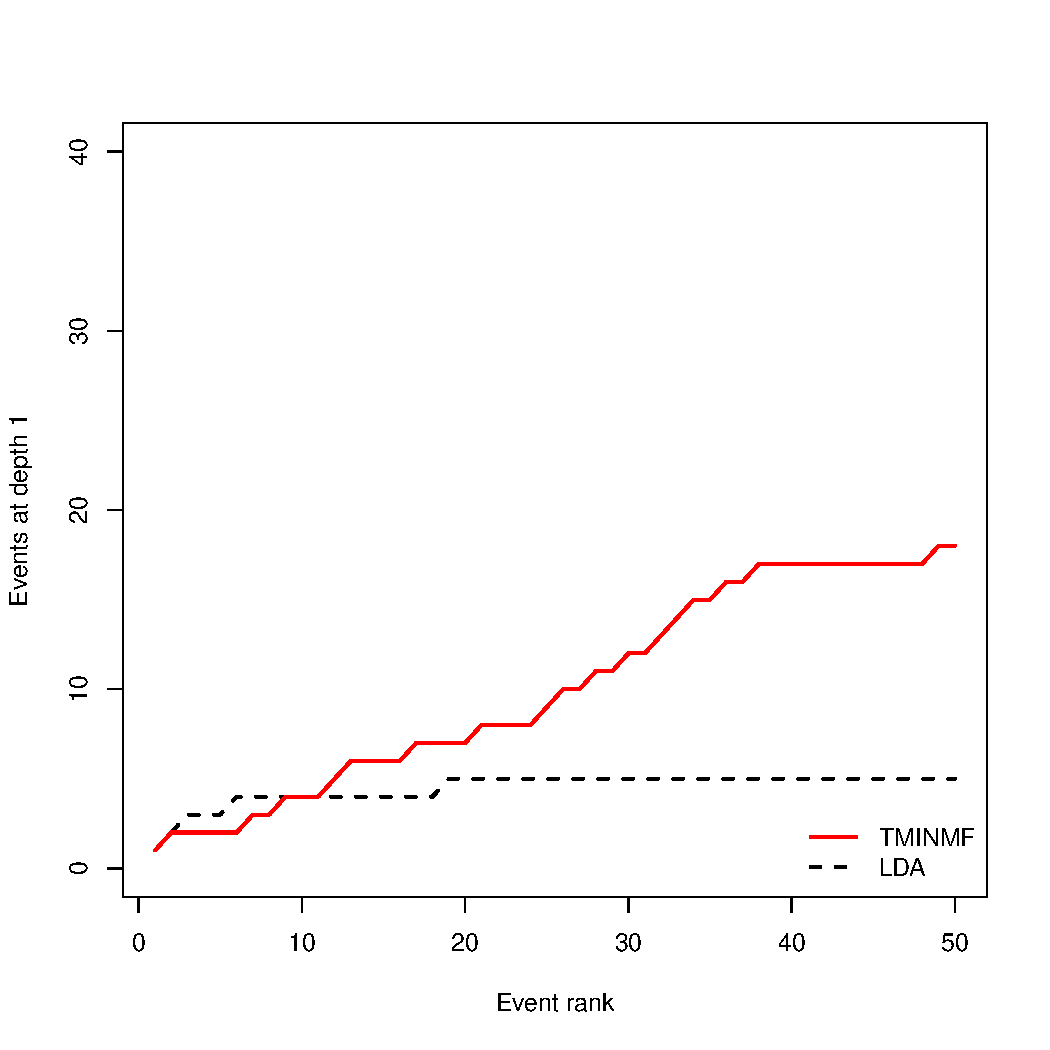
\includegraphics[width=10cm]{plots/events_at_rank_1.pdf}
\end{subfigure}%
\begin{subfigure}{.5\textwidth}
  \centering
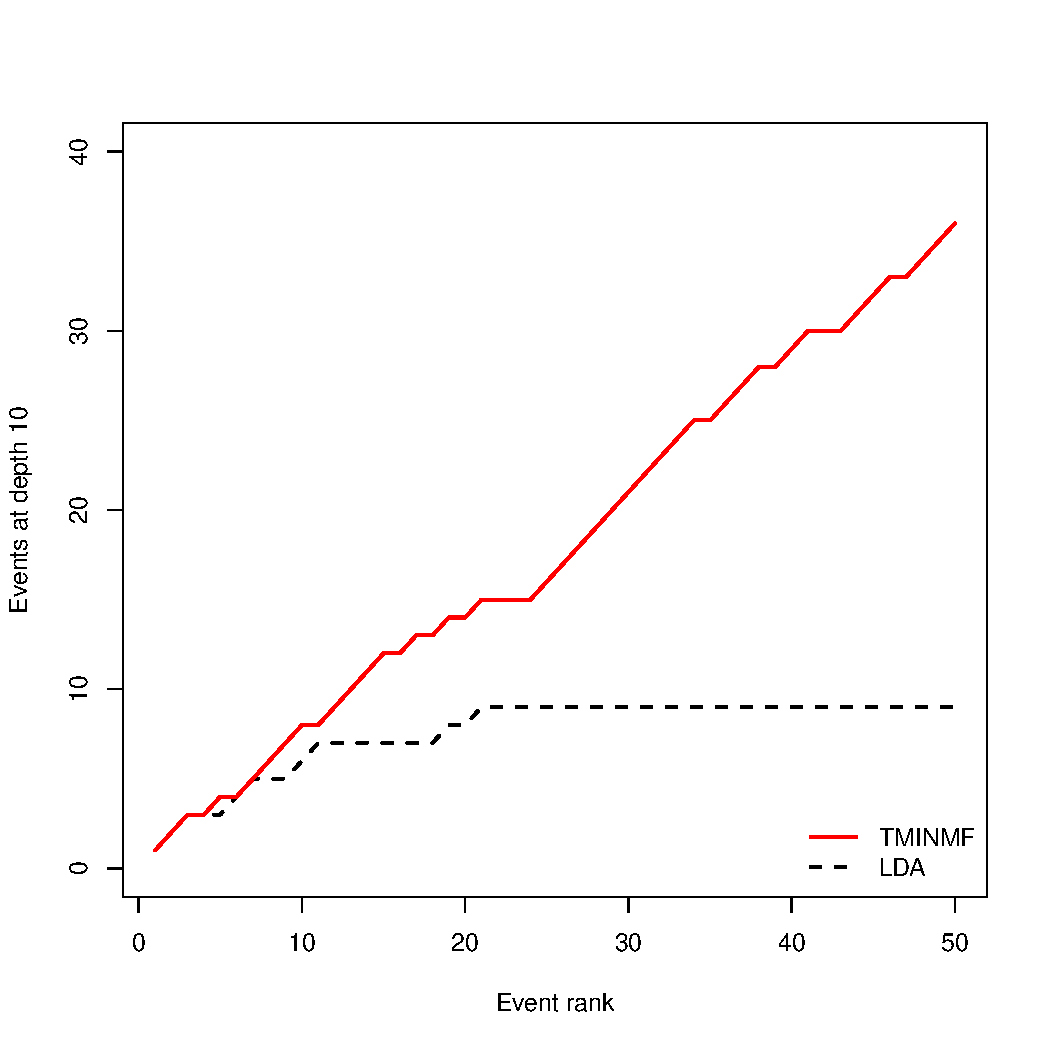
\includegraphics[width=10cm]{plots/events_at_rank_10.pdf}
\end{subfigure}
\caption{(a) number of known-events at each URL depth, (b) number of unique known-event URLs at each depth (c) number of known events at depth 1 for all ranks, (d) number of known events at depth 10 for all ranks.}
\label{fig.eventdist}
\end{figure*}



Overall, we can see that the TMINMF model is more effective at identifying known events 
At depth 10, TMINMF identifies 11 events not identified by LDA
At depth 10, LDA identifies 3 events not identified by TMINMF

Additionally, TMINF identifies several events that have no representation in Wikipedia:


Plots:
* Plot comparing number of candidate events returned at each depth (1-10)
* Plot comparing the number of known-events found at each rank (1-50), possibly for all depths (1-10) or just a fixed depth
* Number of unique known-event URLs returned by each system at depths 1-10



\begin{comment}
\begin{table*}
\small
\begin{tabular}{| l | >{\raggedright}p{7cm} | p{1.5cm} | p{6.3cm} | } \hline
{\bf ID } & {\bf Event model} & {\bf Est. date} & {\bf Top Wikipedia page } \\ \hline
100 & prisoner(0.008) karpinski(0.008) detainee(0.008) sanchez(0.007) taguba(0.007) 205th(0.007) 800th(0.007) fay(0.007) abuse(0.006) prison(0.006),  & 05/19/2004 & Abu\_Ghraib\_torture\_and\_prisoner\_abuse \\ \hline
76 & campaign(0.014) kerry(0.013) 2004(0.012) john(0.009) candidate(0.009) vote(0.008) bush(0.008) senator(0.008) voter(0.007) presidential(0.007) & 10/08/2004 & United\_States\_presidential\_election,\_2004 \\ \hline
91 & sumatra(0.014) tsunami(0.014) indonesia(0.013) aceh(0.012) banda(0.011) deadly(0.01) asia(0.01) lanka(0.01) sri(0.01) earthquake(0.009) & 12/29/2004 & 2004\_Indian\_Ocean\_earthquake\_and\_tsunami \\ \hline
82 & yushchenko(0.012) yanukovich(0.011) kuchma(0.011) kiev(0.01) ukraine(0.009) politics(0.007) viktor(0.007) election(0.007) runoff(0.007) vote(0.007) & 12/05/2004 & Viktor\_Yanukovych \\ \hline
57 & chechen(0.01) moscow(0.009) chechnya(0.009) beslan(0.008) kremlin(0.008) putin(0.008) ossetia(0.008) maskhadov(0.007) basayev(0.007) siege(0.007) & 09/08/2004 & Beslan\_school\_siege \\ \hline
101 & charley(0.012) hurricane(0.012) frances(0.009) storm(0.009) florida(0.007) damage(0.007) ivan(0.007) charlotte(0.006) arcadia(0.006) coast(0.006) & 09/03/2004 &  Hurricane\_Charley \\ \hline
119 & cheney(0.006) edwards(0.006) tempe(0.006) saddam(0.005) format(0.005) hussein(0.005) debate(0.004) kerry(0.004) bremer(0.004) enemy(0.003) & 10/06/2004 & United\_States\_presidential\_election\_debates,\_2004 \\ \hline
112 & vietnam(0.007) convention(0.006) mccain(0.006) swift(0.006) kerry(0.005) swing(0.005) boat(0.005) antiwar(0.005) nominee(0.004) voter(0.004) & 09/02/2004 & Swift\_Vets\_and\_POWs\_for\_Truth \\ \hline
116 & 40th(0.013) reagan(0.011) ronald(0.009) funeral(0.009) gorbachev(0.008) coffin(0.006) alzheimer(0.006) former(0.005) rotunda(0.005) politics(0.005) & 06/09/2004 & Death\_and\_state\_funeral\_of\_Ronald\_Reagan \\ \hline
19 & basque(0.014) spain(0.011) zougam(0.007) qaeda(0.007) morocco(0.006) al(0.006) terrorist(0.005) terrorism(0.005) casablanca(0.005) attack(0.005) & 3/16/2004 & 2004\_Madrid\_train\_bombings \\ \hline
\end{tabular}
\caption{Selected events models, estimated event dates, and the top-ranked Wikipedia page for the NMF model}
\label{table}
\end{table*}

\begin{table}
\begin{tabular}{ | l | l | l | } \hline
			  		& {\bf TMI\/NMF} 	& {\bf He et al. } \\ \hline
N					& 50 		& 50 		\\ \hline
Number of events 		& 33 (0.66) 	&  14 (0.28)	\\ \hline
Unique events 	   		& 27 		&  12		\\ \hline
Events in Wikipedia 		& 25 		&  12	\\ \hline
Mean P@10			& 0.56 		& 0.38 	\\ \hline
\end{tabular}
\caption{}
\label{table}
\end{table}
\end{comment}

\section{Conclusions}

This short paper introduces a novel method for retrospective event detection that relies on three basic steps:
\begin{enumerate}
\item Identification of temporally-interesting terms using time series first-order autocorrelation (ACF)
\item Identification of feature associations using temporal mutual information ($I_t$)
\item Identification of latent event models using non-negative matrix factorization (NMF)
\end{enumerate}

Previous research in the area of retrospective event detection has relied on local evaluation to assess model effectiveness. In this paper, we introduce a preliminary evaluation methodology that can be used for comparative evaluation. Using this evaluation methodology, we demonstrate that our simple model is effective and outperforms a state-of-the-art baseline model.

Points:
This model has a natural way of weighting terms
Terms can be in multiple event models
Temporal MI is better than document overlap for term association	


Future work:
Evaluation over a larger corpus (LDC NYT collection contains articles from 1987-2007)
Estimation and evaluation of event dates
Methods for ranking event importance
Generative model (Topics over Time)

\section{Acknowledgments}
This work was supported in part by the US National Science Foundation under Grant No. [blind]. Any opinions, findings, conclusions, or recommendations expressed are those of the authors and do not necessarily reflect the views of the National Science Foundation.


\bibliographystyle{abbrv}
\bibliography{eventdetection}  

\end{document}
